\documentclass{standalone}
\usepackage{pgfplots}
\pgfplotsset{compat=1.5}
\usepgfplotslibrary{fillbetween}
\usetikzlibrary{shapes,positioning,intersections,quotes,patterns}

\pgfplotsset{soldot/.style={color=black,only marks,mark=*}} 
\pgfplotsset{holdot/.style={fill=white,mark=*}}

\begin{document}

\centering
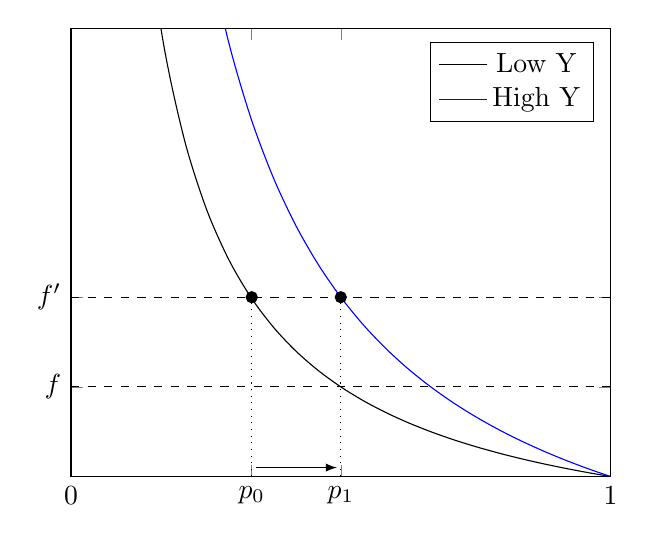
\begin{tikzpicture}
\begin{axis}[
%xlabel={$p$},
%ylabel={$f$},
smooth,
legend pos=north east,
xmin=0,
xmax=1,
ymin=0,
ymax=5,
ytick={1,2},
yticklabels={$f$,$f^\prime$},
xtick={0,0.335,0.5,1},
xticklabels={0,$p_0$,$p_1$,1},
restrict y to domain=0:10,
]

% Plots
\def\a{1}
\def\Y{1}
\def\yy{2}
\def\O{0}

\addplot[name path=F,domain=0:1,solid, black] {(((1-x)*\Y^\a-\O^\a)/x)^(1/\a)};
\addlegendentry{Low Y}
\addplot[name path=F,domain=0:1,solid, blue] {(((1-x)*\yy^\a-\O^\a)/x)^(1/\a)};
\addlegendentry{High Y}

% Shading
%\addplot[fill=gray!25]fill between[of=F and G, soft clip={domain=0:1}];
%\addplot[fill=gray!25]fill between[of=M and G, soft clip={domain=0:0.17}];
%% Correcting vertical axis that got covered by shade
%\draw[] (axis cs:0,0) -- (axis cs:0,5);

% Values of probability of detection
%\draw[dashed] (axis cs:0.2,0) -- (axis cs:0.2,2);
\draw[dotted] (axis cs:.335,0) -- (axis cs:.335,2);
\draw[dotted] (axis cs:0.5,0) -- (axis cs:0.5,2);

% Fines
\addplot[domain=0:1,dashed,mark=none,black] {1};
\addplot[domain=0:1,dashed,mark=none,black] {2};
%\addplot[soldot] coordinates{(0.2,2)} node[above](){};
\addplot[soldot] coordinates{(0.335,2)} node[above](){};
\addplot[soldot] coordinates{(0.5,2)} node[above](){};

\draw[>=latex,shorten >=0.05cm,shorten <=0.05cm, black,->] (axis cs:0.335,0.1)--(axis cs:0.5,0.1);


\end{axis}
\end{tikzpicture}

\end{document}